\begin{center}
\vspace{0.5pt}\nointerlineskip\rule{\textwidth}{0.2pt}\\ 
\vspace{0.5pt}\nointerlineskip
\end{center} 
\large Datum: 15.04.2019\vspace{3pt}\\\large Protokollant/in: Marian Geißler
\section{Themen}
\begin{LARGE}
Sprint 2 Auswertung\\
\end{LARGE}
Ticket: Testdatensatz von Marian - Testdatensatz soll in zukünftigen Sprints für gesamtes Programm automatischen Ausgabe-Test verwendet werden\\
Ticket: SWT für Linux - deleted\\
Ticket: Pfadbehandlung unter Windows - abgeschlossen\\
Ticket: Codecollector einlesen  \\
Ticket: BugfixParser - Bugs bestehen weiterhin. Wird in nächsten Sprint mit aufgenommen\\
Ticket: Unit Test für gesammtes Programm\\
Ticket: Parser für Sequenzdiagramme\\
Ticket: Ausgabe für Sequensdiagramme\\
Es folgten Vorgaben für xml-Konfiguration zur strukturierten Datendarstellung\\
Evtl. Idee eines ausgelagerten Parsers nur für Funktionen.\\
\begin{LARGE} 
Planung Sprint 3\\
\end{LARGE}
Neue Aufgaben: GUI zu AWT/Swing umbauen\\
Parser soll weiterhin optimiert werden\\
Neues Ziel: Entwicklung Richtung XML als Basis erweitern\\
Parser soll zukünftig XML-Stream liefern\\
Parser mit Option für Sequenzdiagramme\\
\section{Ergebnisse/Vereinbarungen}
\begin{figure}
	\centering
	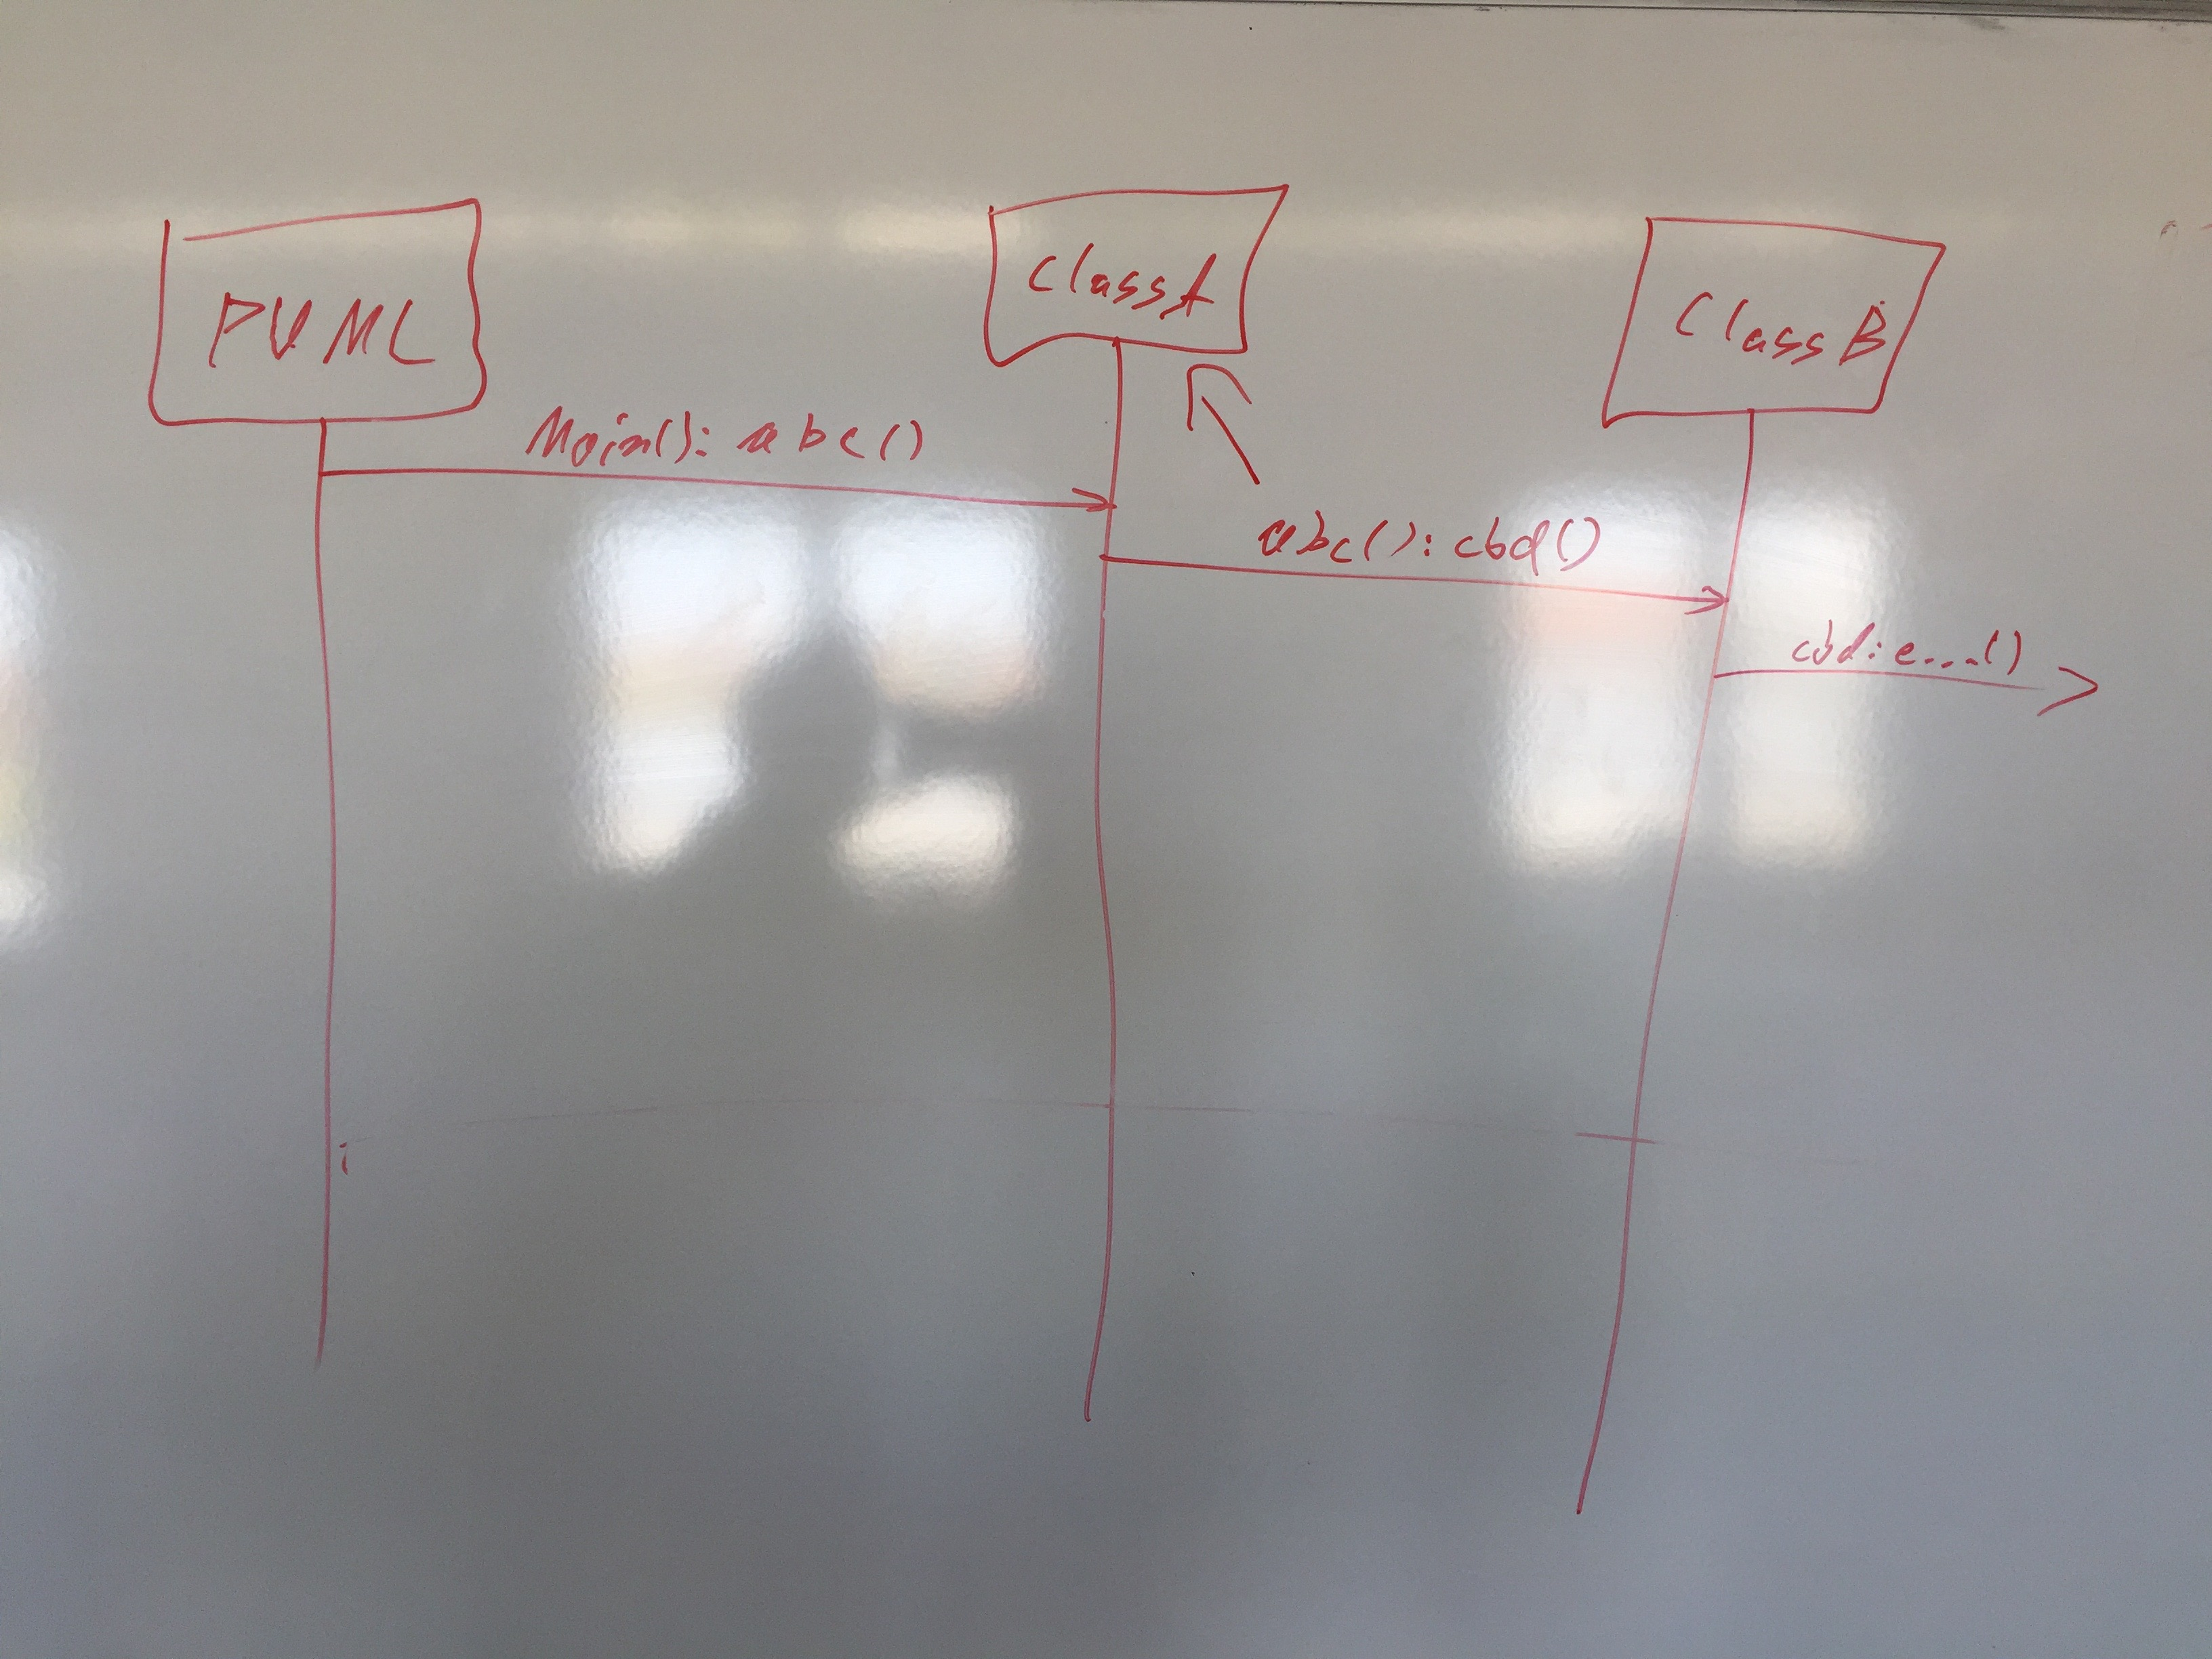
\includegraphics[width=8cm]{bilderMinutes/sequenceDiagrammFkt_Tafel}
	\caption{Tafelbild SQDiagramm}
\end{figure}
\begin{itemize}
\item Sprint 2 beendet\\
\item UTF-8 als Standard einhalten\\
\item Neuer Development-Branch \\
\item Swing als neuer Standard für GUI werden\\
\end{itemize}
\section{Hinweise}
Nächste Zwischenstands-Präsentation am Mo,06.05.2019 um 12:45
\section*{Nächstes Treffen:}
25.04.2019 um 11:15